%
\label{sec:structure}

%\fitter is a flexible open-source platform for the QCD analyses of different experimental measurements, 
%providing a versatile environment for benchmarking studies. It is widely used within the
%LHC experiments~\cite{atlas:strange,atlas:jets,atlas:hm,cms:strange,h1:2012kk,h1zeus:charm}.  

In this section the functionality of \fitter is described.
A block diagram in Fig \ref{fig:flow} gives a schematic view
of the \fitter functionality which can be divided into four main blocks:
\begin{figure}[!ht]
  \begin{tikzpicture}[node distance=1cm, auto,>=latex', thick]
      \path[->] node[draw, text width=2cm, align=center] at (0,0) (init) {\bf Initialization};
      \path[->] node[draw, below left=0.3cm and -0.7cm of init, text width=3.5cm] (data) 
                    {\begin{center} \vspace{-0.3cm}{\bf Input Data} 
		      \\ {\color{blue}\small Data Type} 
		     \end{center} 
		     {\scriptsize 
		     \begin{itemize}
                      \vspace{-0.3cm}
		      \item Collider ep
		      \item Collider pp
		      \item Fixed target data
		     \end{itemize}}
		     } (init) edge (data);
      \path[->] node[draw, below right=0.3cm and -0.7cm of init, text width=3.5cm] (theory) 
                    {\begin{center} \vspace{-0.3cm}{\bf Theory Predictions} 
		      \\ {\color{red}\small Factorization Theorem} 
		     \end{center} 
		     {\scriptsize 
		     \begin{itemize}
                      \vspace{-0.3cm}
		      \item PDF Parametrisation
		      \item QCD Evolution (QCDNUM)
		      \item Cross Section Calculation
		     \end{itemize}}
		     } (init) edge (theory);
      \path[->] node[draw, below right=0.4cm and -1.4cm of data, text width=3.5cm] (minuit) 
                    {\begin{center} \vspace{-0.3cm}{\bf Minimisation (MINUIT)} 
                      \vspace{-0.2cm}
		     \end{center} 
		     {\color{blue}\scriptsize Treatment of the uncertainties:} 
		     {\scriptsize 
                      \vspace{-0.1cm}
		     \begin{itemize}
		      \item PDF Parametrisation
		      \item QCD Evolution (QCDNUM)
		      \item Cross Section Calculation
		     \end{itemize}}
		     } (data) edge (minuit)
		     (theory) edge (minuit)
		     (data) ++ (1.6,0) edge [<->,double equal sign distance] ++(1.36,0) (theory);
      \path[->] node[draw, below =0.4cm  of minuit, text width=3.5cm] (res) 
                    {\begin{center} \vspace{-0.3cm}{\bf Results} 
		     \end{center} 
		     {\scriptsize 
		     \begin{itemize}
                      \vspace{-0.3cm}
		      \item PDF LHgrids
		      \item alphas, mc, \dots
		      \item Data vs Predictions
		      \item \(\chi^2\), pulls, shifts
		     \end{itemize}}
		     } (minuit) edge (res);
  \end{tikzpicture}
  \caption{Schematic structure of the \fitter program.} 
  \label{fig:flow}
\end{figure}

%\begin{figure}[!ht]
%   \centering
%   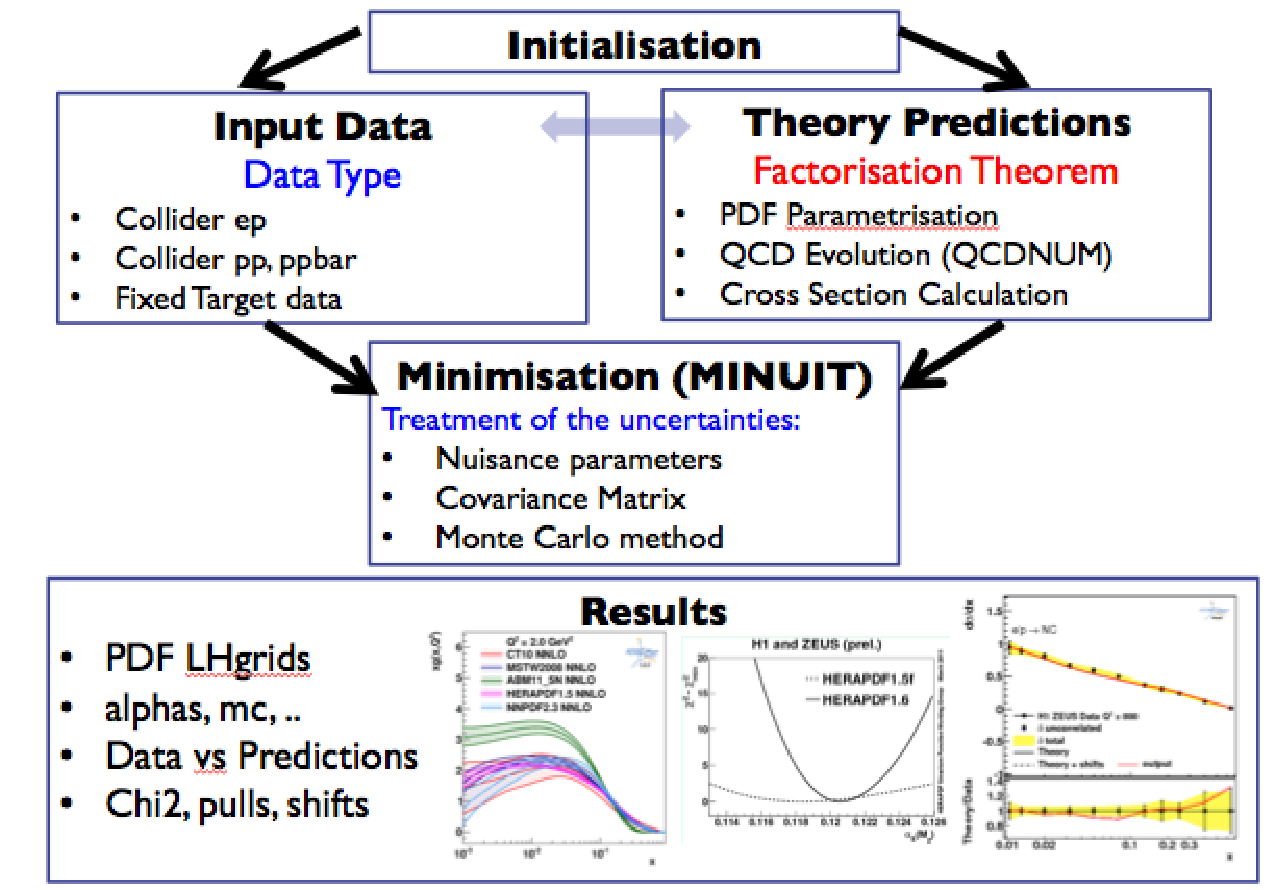
\includegraphics[width=8cm]{flow.pdf}
%   \caption{Schematic structure of the \fitter~program.} 
% \label{fig:flow}
%\end{figure}
%\begin{description}
%\item 
\paragraph{Data:} Different measurements from various processes
are implemented in the \fitter package including the full information on their uncorrelated 
and correlated uncertainties. HERA inclusive scattering data 
are sensitive to quark PDFs and to gluon PDFs through scaling violations and the longitudinal structure function $F_L$.  
%covering low and medium $x$ ranges. 
These data are the backbone of any proton PDF extraction,
and are used by all global PDF groups \cite{MSTWpdf,CT10pdf,NNPDFpdf,Alekhin:2013nda,Jimenez-Delgado:2014twa}.  They can be supplemented by HERA measurements sensitive to heavy quarks and by HERA jet measurements, which have sensitivity to the gluon PDF.
However, the kinematic range of HERA data mostly covers low and medium $x$ ranges.
Improvements in precision of PDFs require additional constraints on the gluon and 
quark distributions at high-$x$, better understanding of heavy quark distributions and 
decomposition of the light-quark sea.  For these purposes, measurements from the fixed-target 
experiments, the Tevatron and the LHC can be used.
% are of particular importance.
%
%Additional measurements provide constraints to the sea flavour decomposition, such as the new 
%results from the LHC, as well as constraints to PDFs in the kinematic phase-space regions 
%where HERA data is not measured precisely, such as the high $x$ region for the gluon and valence 
%quark distributions from Tevatron and fixed target experiments.
%
The processes that are currently available in \fitter framework are listed in Tab.~\ref{tab:proc}.

%
\begin{table}
\small
%\tiny
\scriptsize

\begin{tabular}{|l|l|l|l|}
\hline 
\textbf{Experimental} &\textbf{Process}&\textbf{Reaction}&\textbf{Theory} \\
\textbf{Data}         &        &                &\textbf{calculations, schemes}  \\
\hline \hline \\ [-2.5ex]
%\multirow{6}{*}{HERA} &DIS NC   &$ep\to eX$      & TR', ACOT \\
HERA, &DIS NC   &$ep\to eX$      & TR$^\prime$, ACOT, \\
Fixed Target     &         &                & ZM (\qcdnum), \\
     &         &                & FFN (\texttt{OPENQCDRAD}, \\
     &         &                & \qcdnum), \\ 
     &         &                & TMD (uPDFevolv) \\ [0.5ex]
\hline \\ [-2.5ex]
%\cline{2-4}  \\ [-2.0ex]
HERA &DIS CC   &$ep\to \nu_e X$ & ACOT, ZM (\qcdnum), \\
     &         &                & FFN (\texttt{OPENQCDRAD)} \\  [0.5ex]
\cline{2-4}  \\ [-2.0ex]
     &DIS jets &$ep\to e\ \mathrm{jets}X$      & \nlojetpp (\fastnlo)\\ [0.5ex]
\cline{2-4} \\ [-2.0ex]
     &DIS heavy quarks & $ep\to e c \bar{c} X$, & ZM (\qcdnum), \\
     &         & $ep\to e b \bar{b} X$ & TR$^\prime$, ACOT, \\
     &         &                & FFN (\texttt{OPENQCDRAD}, \\
     &         &                & \qcdnum) \\  [0.5ex]
\hline \\ [-2.5ex]
%Fixed Target   &DIS NC          &$ep\to eX$ & ZM (\qcdnum), \\
%     &         &                & TR', ACOT, \\ [0.5ex]
%     &         &                & FFN (\texttt{OPENQCDRAD}, \\
%     &         &                & \qcdnum) \\  [0.5ex]
%\hline \\ [-2.5ex]
Tevatron,&Drell-Yan &$pp(\bar p)\to l\bar l X$, & \mcfm (\applgrid) \\
LHC              &          &$pp(\bar p)\to l\nu  X$ &                 \\ [0.5ex]
\cline{2-4}  \\ [-2.0ex]
%Tevatron, LHC &W charge asym &$pp(\bar p) \to l\nu X$ & MCFM (\texttt{APPLGRID}) \\
%\hline
              &top pair   &$pp(\bar p) \to t\bar t X$  & \mcfm (\applgrid),  \\
              &            &                            & \texttt{HATHOR}      \\  [0.5ex] 
\cline{2-4}  \\ [-2.0ex]
              &single top &$pp(\bar p) \to t l \nu X$,      & \mcfm (\applgrid) \\
              &           &$pp(\bar p) \to tX$,             &  \\
              &           &$pp(\bar p) \to tWX$             &  \\ [0.5ex]
\cline{2-4}  \\ [-2.0ex]
             &jets &$pp(\bar p) \to \mathrm{jets} X$ & \nlojetpp (\applgrid), \\
                &  & & \nlojetpp (\fastnlo) \\ [0.5ex]
\hline  \\ [-2.5ex] 
LHC& DY+heavy quarks &$pp \to VhX$ & \mcfm (\applgrid) \\  [0.5ex]
\hline
\end{tabular}
\caption{The list of experimental data and theory calculations implemented in the \fitter package. 
The references for the individual calculations and schemes are given in the text.
}
%The APPLGRID~\cite{Carli:2010rw} and FastNLO~\cite{Kluge:2006xs,Wobisch:2011ij,Britzger:2012bs} 
%techniques for the fast interface to theory calculations are described in section~\ref{sec:techniques}.} 
\label{tab:proc}
\end{table}
%
\normalsize
%\item
\paragraph{Theory:}  
%Predictions for cross section of different processes are obtained using 
%the factorisation approach (Eq.~\ref{eq:fact}).
 The PDFs are parametrised at a starting input scale, $Q_0^2$,  
by a chosen functional form with a set of free parameters $\vec{p}$. 
These PDFs are evolved to the scale of the measurement $Q^2$, $Q^2>Q_0^2$.
The evolution uses the DGLAP formalism \cite{Gribov:1972ri, Gribov:1972rt, Lipatov:1974qm,
Dokshitzer:1977sg, Altarelli:1977zs} (as implemented in \qcdnum~\cite{qcdnum}) by default, however CCFM evolution \cite{\CCFM} is also available 
(as implemented in \texttt{uPDFevolv}~\cite{tmdlref2}).
%or dipole models~\cite{Golec-Biernat:1998js,Iancu:2003ge,Bartels:2002cj}.
The prediction of the cross section for a particular process is obtained, assuming factorisation,  by the convolution of the evolved 
PDFs and the appropriate hard-process parton scattering cross section.
Appropriate theory calculations are listed in Tab.~\ref{tab:proc}.
Alternatively, predictions using dipole models~\cite{Golec-Biernat:1998js,Iancu:2003ge,Bartels:2002cj} can also be obtained.
%\item
\paragraph{QCD Analysis:} \rm  
The PDFs are determined by a least square fit, minimising a $\chi^2$ function, constructed using the input data and theory predictions, with the \minuit \cite{minuit} program.
%with respect to free parameters $\vec{p}$ using the MINUIT~\cite{minuit} program.
%
%extracted from a least square fit by minimising the  $\chi^2$ function with respect to free parameters. 
%The $\chi^2$ function is formed from the input data and the theory prediction.
%The $\chi^2$ is  minimised iteratively 
%with respect to$\vec{p}$ using the MINUIT~\cite{minuit} program.
In \fitter various choices are available to account for the experimental uncertainties. Correlated experimental uncertainties can be accounted for using 
a nuisance parameter method  
or a covariance matrix method as described in section~\ref{sec:chi2representation}.  Different statistical assumptions for the distributions of the systematic uncertainties, like Gaussian or LogNormal~\cite{hera-lhc:report2009} can also be studied (see section~\ref{sec:experimentalerrors}).
%\item
\paragraph{Results:}
%The fitted parameters $\vec{p}$ and their estimated uncertainties are produced. 
The resulting PDFs are provided in a format ready to be used by the \lhapdf 
library~\cite{lhapdf,lhapdfweb} or by \tmdlib \cite{tmdlref}.
\fitter drawing tools can be used to display the PDFs with their uncertainties at a chosen scale.  
%Drawing tools are supplied which allow the PDFs to be
%graphically  displayed at chosen scales by the users with their one sigma uncertainty bands. 
As an example, the first set of PDFs extracted using \fitter from HERA I data, HERAPDF1.0 \cite{h1zeus:2009wt}, 
is shown in Fig.~\ref{fig:hera1} (taken from \cite{h1zeus:2009wt}).
 Note that the PDFs displayed are parton momentum distributions $xf(x,\mu_F^2)$ since this is how PDFs are conventionally stored and displayed.
%%%Since then several other PDF sets were produced within the HERA \cite{hera:grids} and LHC \cite{atlas:grids} collaborations.
%In addition to the PDF display, 
%The comparison of data used in the fit to the theory predictions are also produced. 
% plots which compare the input data to the fitted theory predictions can be produced 
%to demonstrate the fit consistency. 
\begin{figure}[!ht]
   \centering
   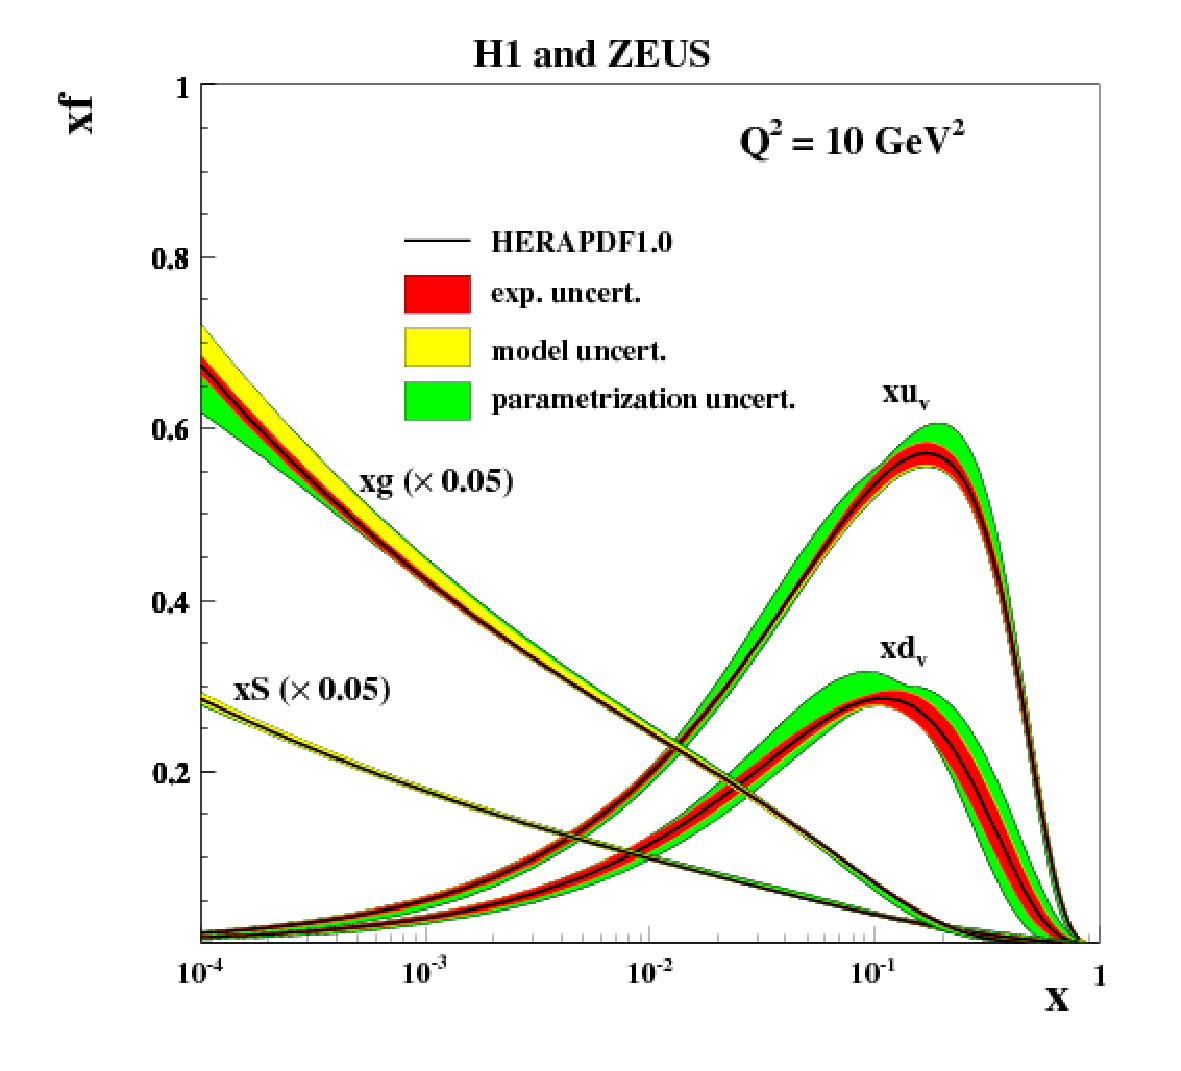
\includegraphics[width=8cm]{hera1.pdf}
   \caption{Distributions of valence ($xu_v$, $xd_v$), sea ($xS$) and the gluon ($g$) densities in HERAPDF1.0~\cite{h1zeus:2009wt}. 
       The gluon and the sea distributions are scaled down by a factor of 20.
       The experimental, model and parametrisation uncertainties are shown as coloured bands.}
       %Summary plots of valence ($xu_v$, $xd_v$), total sea ($xS$, scaled) and gluon ($xg$, scaled) densities
       %with their experimental, model and parametrisation uncertainties shown as colored bands at the scale 
       %of $Q^2=10 \ \GeV^2$ for the HERAPDF1.0 PDF set~\cite{h1zeus:2009wt}.}
 \label{fig:hera1}
\end{figure}
%In Fig.~\ref{fig:data}, a comparison of inclusive NC data from the HERA~I running period with predictions based on HERAPDF1.0 is shown. 
%The inclusive NC data from the HERA I are compared with the predictions based on 
%HERAPDF1.0 PDFs in Fig.~\ref{fig:data}.


%Also shown are theory predictions, obtained using the nuisance parameter method, 
%which accounts for correlated systematic
%shifts when using the nuisance parameter method that accounts for 
%correlated systematic uncertainties (see section~\ref{sec:chi2representation}). 
%The consistency of the measurements and the theory is expressed by pulls, defined as a difference between data 
%and theory divided by the uncorrelated error of the data. 
%In each kinematic bin of the measurement, pulls are provided in units of standard deviation (sigma).  
%As an additional consistency check between data and the theory predictions, pull information, defined as the difference between data and prediction divided by the uncorrelated uncertainty of the data, is displayed in units of sigma shifts for each given data bin.
%\begin{figure}[!ht]
%   \centering
%   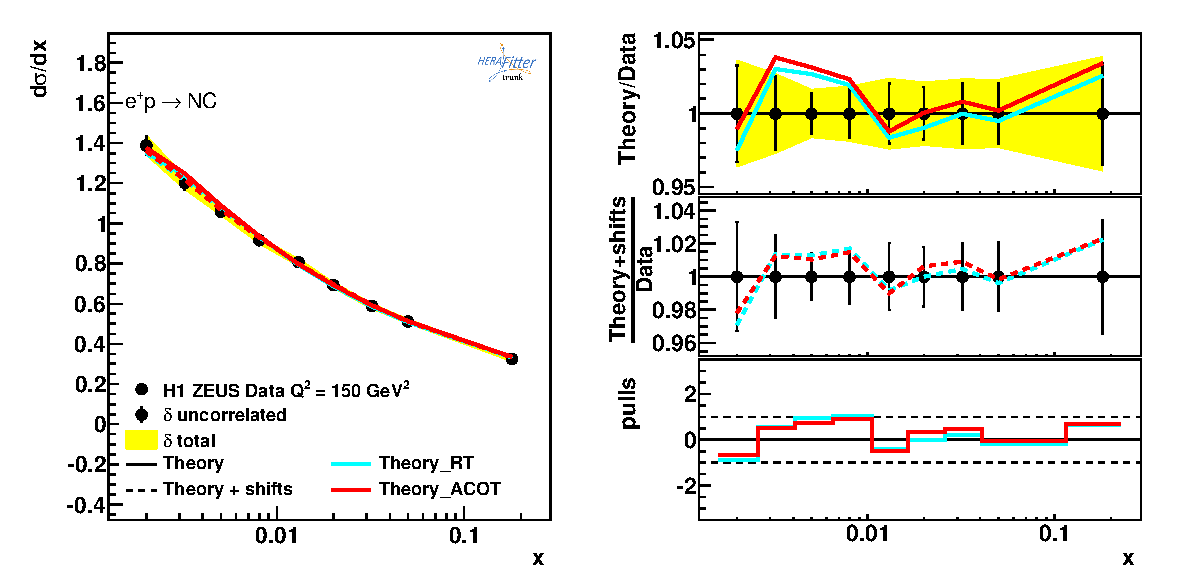
\includegraphics[width=8.6cm]{datatheory.pdf}
%   \caption{An illustration of the consistency of HERA measurements~\cite{h1zeus:2009wt} and the theory predictions, 
%       obtained in \fitter with the default drawing tool.} 
%       %In addition, ratio plots are also provided together with the pull distribution (right panel).}    
% \label{fig:data}
%\end{figure}

%\end{description}
%
%This paper provides a comprehensive description of  \\
%the \fitter\ package.
%which is designed for analysis of the High Energy Physics data.
%The package has been developed by members of the H1 and ZEUS collaborations
%with an exclusive support of different theoretical groups.
%The main purpose of the \fitter\ package is analysis of the 
%data from the $e^{\pm}p$, $p\bar{p}$, and $pp$ collider experiments
%information obtained from the deep inelastic scattering experiments
%and the determination of the parton density functions (PDFs).
%The broad range of data taken from the $e^{\pm}p$, $p\bar{p}$, and $pp$ collider experiments can be
%studied by the package. 

%Based on the concept of factorisable nature of the cross sections into universal parton distribution functions (PDFs) and process dependent partonic scattering cross sections, 

%The \fitter\ program facilitates the determination of the PDFs from many 
%cross section measurements at $ep$, $p\bar{p}$ or $pp$ colliders.  
% It includes various options for theoretical calculations and various choices 
%of how to 
%account for the experimental uncertainties. 
%The \fitter project provides a versatile environment for benchmarking studies 
%and a flexible platform for the QCD interpretation of analyses within the LHC experiments,
%as already demonstrated by several publicly available results using the \fitter 
%framework~\cite{atlas:strange,atlas:jets,atlas:hm,cms:strange,cms:jets,h1:2012kk,h1zeus:charm}.  
